\documentclass{article}
\usepackage{graphicx}
\usepackage{geometry}
\usepackage{amsmath}
\geometry{a4paper,
	      total={160mm,247mm},
	      left=25mm,
	      top=25mm}

\title{HSPO: Quantized D-controlled negative damping oscillator demonstration}
\date{23/08/2018}
\author{Gergely Gyebrószki}

\begin{document}
	
\maketitle

\noindent\texttt{COCO version: 2017 Nov 18}

\section{Problem description}

Consider an 1 DoF (degree of freedom) negative damping oscillator with continuous D-control and unit quantization at the calculated control effort. The quantization rounds the control efforts toward zero, therefore it creates a deadzone ($\mathrm{abs}(\dot{x})<1$), where the control is turned off.
The linearized equation of motion is:

\begin{equation}\label{eq:1}
	\ddot{x}-2\,\delta\,\alpha\,\dot{x}+\alpha^2\,x = \mathrm{Int}(D\,\dot{x}),
\end{equation}
where $\alpha$ is the natural frequency, and $\delta$ is the amount of negative damping.

For the sake of simplicity, let the control gain be $D=1$ and examine the state space range $\mathrm{abs}(\dot{x})<2$, where the control effort is either 0, or $\pm$1.
Rewriting Eq. (\ref{eq:1}) as a system of first order ODEs:
\begin{eqnarray}
\dot{v} &=& 2\,\delta\,\alpha\,v - \alpha^2\,x - M \\
\dot{x} &=& v, \nonumber
\end{eqnarray}
where
\begin{equation}
	M=
	\begin{cases}
	\mathrm{sign}(v), & \mathrm{abs}(v) \geq 1\\
	0 & otherwise\\
	\end{cases}
\end{equation}
Let $M^+$ denote the switching line at $v = 1$ and $M^-$ denote the switching line at $v = -1$.
Based on the system parameters, 4-segment periodic orbits or 6-segment periodic orbits (with sliding on the switching lines) can occur.
During sliding, the trajectory is pushed towards a switching line from both sides and the dynamics is reduced to:
\begin{eqnarray}
\dot{v} &=& 0\\
\dot{x} &=& v. \nonumber
\end{eqnarray}
Sliding mode ends when the \emph{uncontrolled} dynamics yields $\dot{x} \leq 0$.\\
Our goal is to generate a family of periodic orbits using \textsc{coco} and its \textsc{po} toolbox.


\section{Implementation and solution using \textsc{coco}}
This system is implemented in \texttt{Oscillator.m}, see \texttt{f(x, p, mode)} and \texttt{events(x, p, event)} functions. The oscillator has three modes: \emph{uncontrolled} (U) when $M=0$, \emph{controlled} (C) when $M=\pm1$ and \emph{sliding} mode (S).

For $\alpha = 1.5$, $\delta = 0.2$, an initial guess for a 4-segment periodic orbit (starting at $[v, x]= [-1, -0.87]$) is obtained using \textsc{Matlab}'s \texttt{ode45}. See Section 1 of \texttt{hspo\_varying\_segment\_demo.m} and Fig. \ref{fig:1}.

\begin{figure}[h!]
	\centering 
	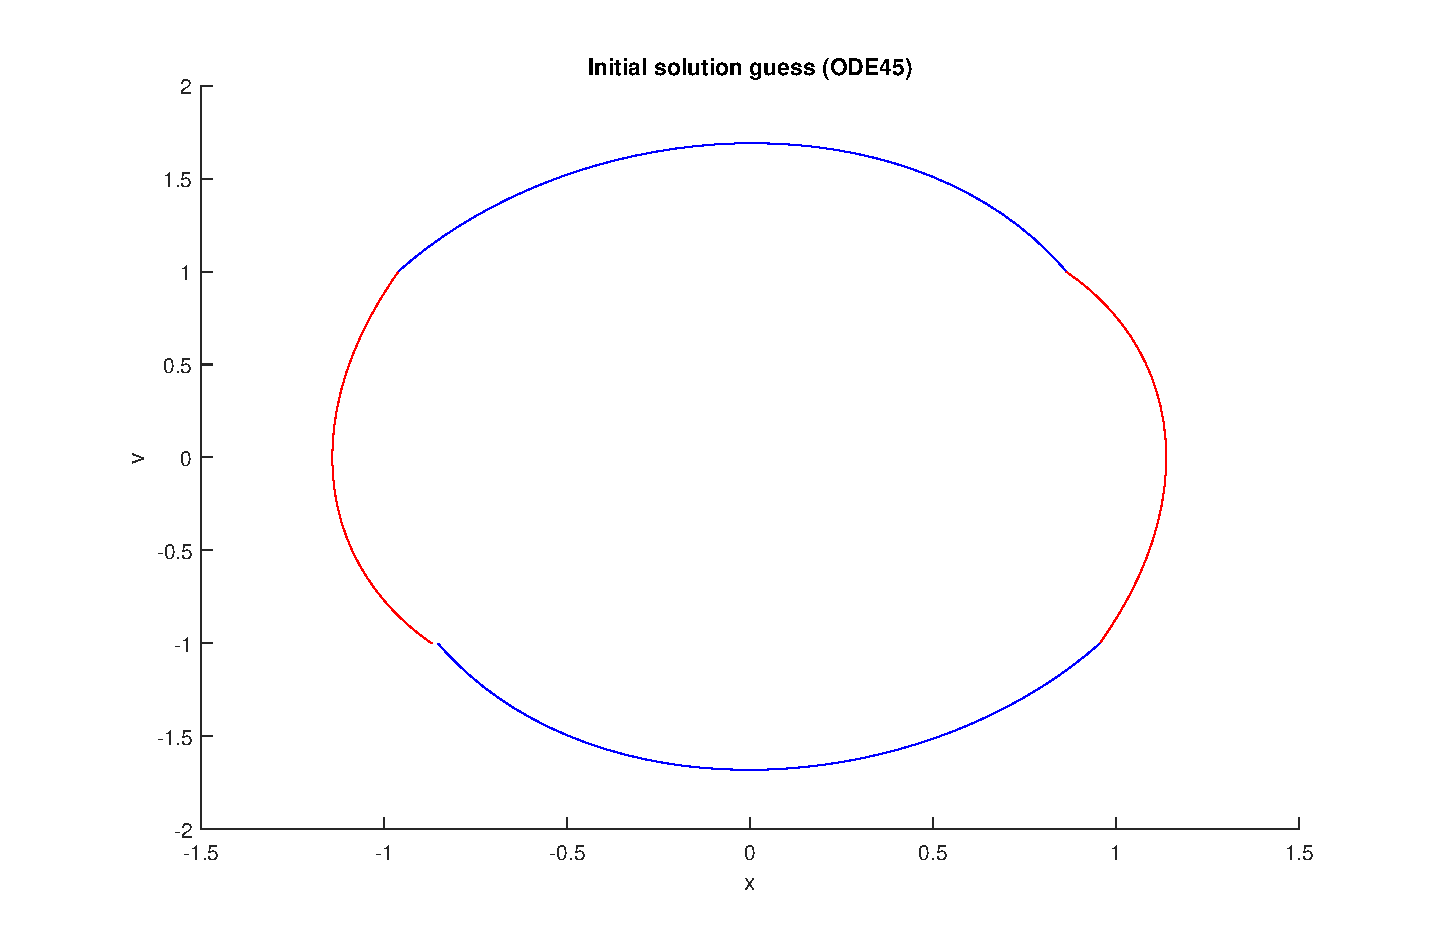
\includegraphics[height=8cm]{fig1}
	\caption{Initial solution guess for a \emph{UCUC} PO. \label{fig:1}}
\end{figure}

\newpage 
This initial solution can be converted to a \textsc{coco} problem using the \texttt{ode\_isol2hspo} constructor. For the four segments the corresponding modes are \emph{uncontrolled, controlled, uncontrolled, controlled} (or shortly \emph{UCUC}), the corresponding events are hitting $M^+$ from below, then $M^+$ from above, hitting $M^-$ from above, and lastly $M^-$ from below. (Or shortly $M^+M^+M^-M^-$). A monitor function is also added to check the condition of sliding mode. (See \texttt{Oscillator.monitor\_sliding\_begins})

The continuation is executed in Section 2 of \texttt{hspo\_varying\_segment\_demo.m}, which generates Fig. \ref{fig:2}. 

\begin{figure}[h!]
	\centering 
	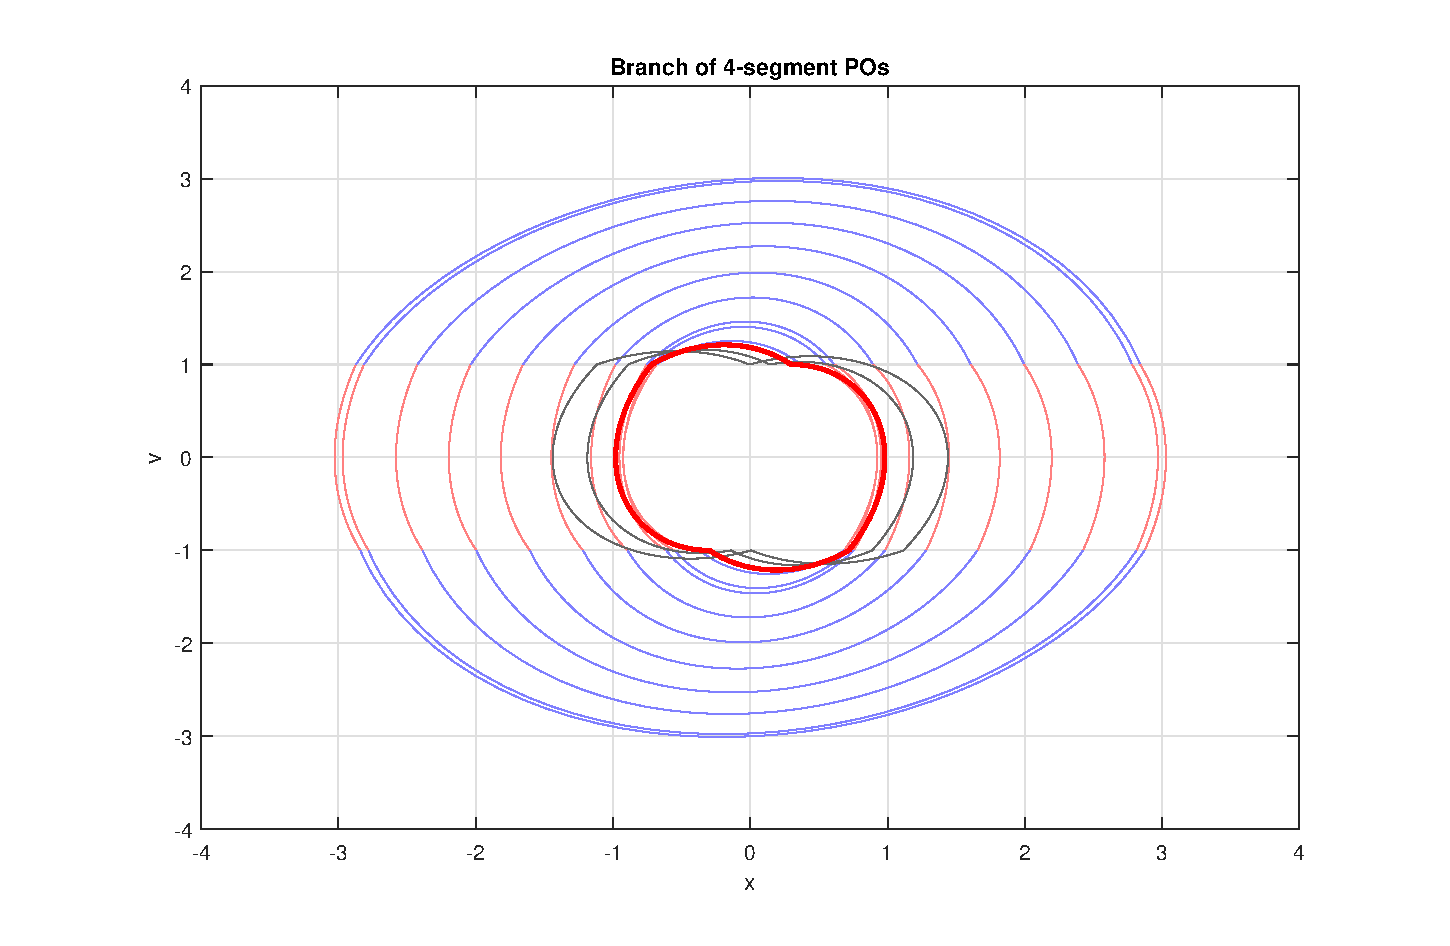
\includegraphics[height=8cm]{fig2}
	\caption{Family of 4-segment \emph{UCUC} POs. Red colour indicates the event where sliding mode begins, gray POs are nonphysical orbits (\emph{uncontrolled} segment re-enters the controlled zone).\label{fig:2}}
\end{figure}

Starting from the highlighted red PO on Figure \ref{fig:2}, a $UCSUCS$ 6-segment PO is constructed, where the \emph{sliding} (S) segments are single points. See Section 3 of \texttt{hspo\_varying\_segment\_demo.m}. \textsc{coco} expands the \emph{sliding} segments and continues a family of 6-segment POs. An event corresponding to the disappearance of the (C) segments are also added. (See \texttt{Oscillator.monitor\_ctrl\_disappears}.) The results are shown on Figure \ref{fig:3}.

\begin{figure}[h!]
	\centering 
	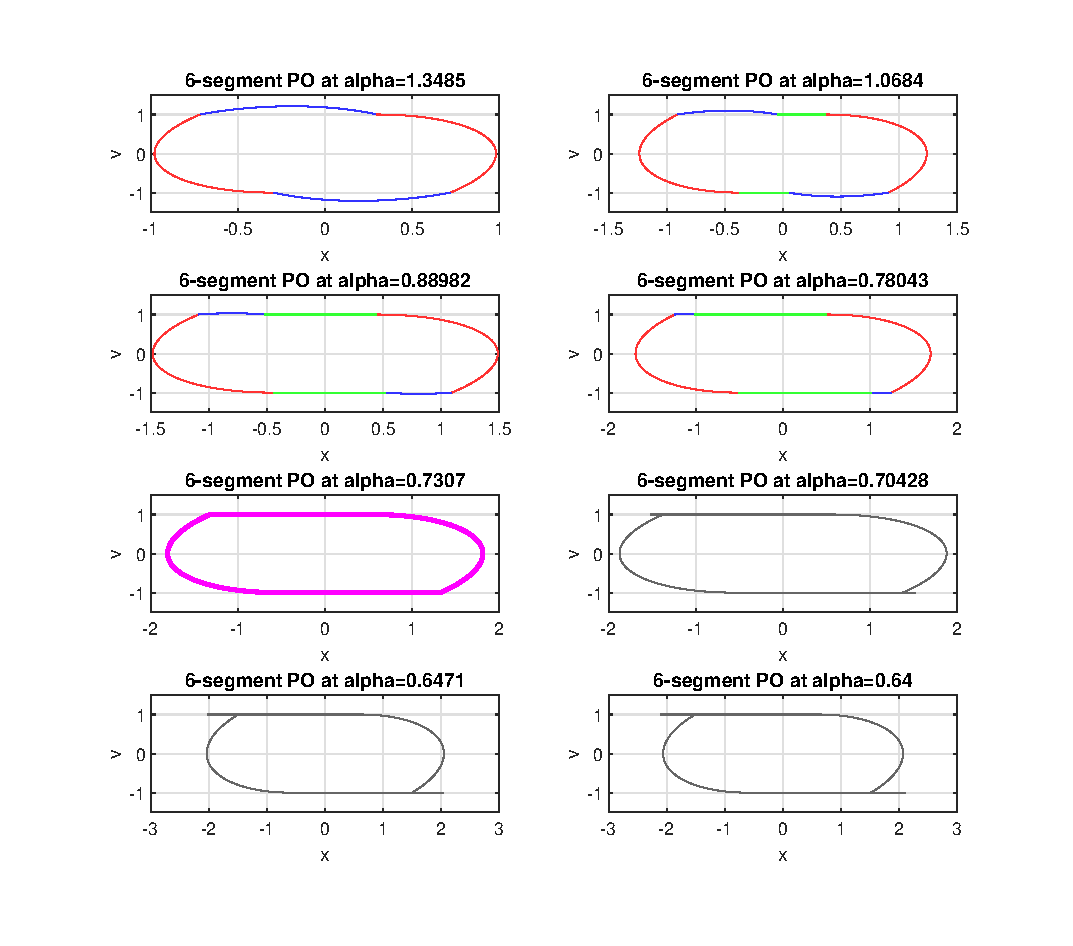
\includegraphics[height=10cm]{fig3}
	\caption{Family of 6-segment \emph{UCSUCS} POs. Pink colour indicates the event where the \emph{controlled} segments disappear, gray POs are nonphysical orbits.\label{fig:3}}
\end{figure}
\newpage 
Lastly, starting from the pink PO, a family of 4-segment \emph{USUS} POs are continued. This is carried out in Section 4 of \texttt{hspo\_varying\_segment\_demo.m}.

\begin{figure}[h!]
	\centering 
	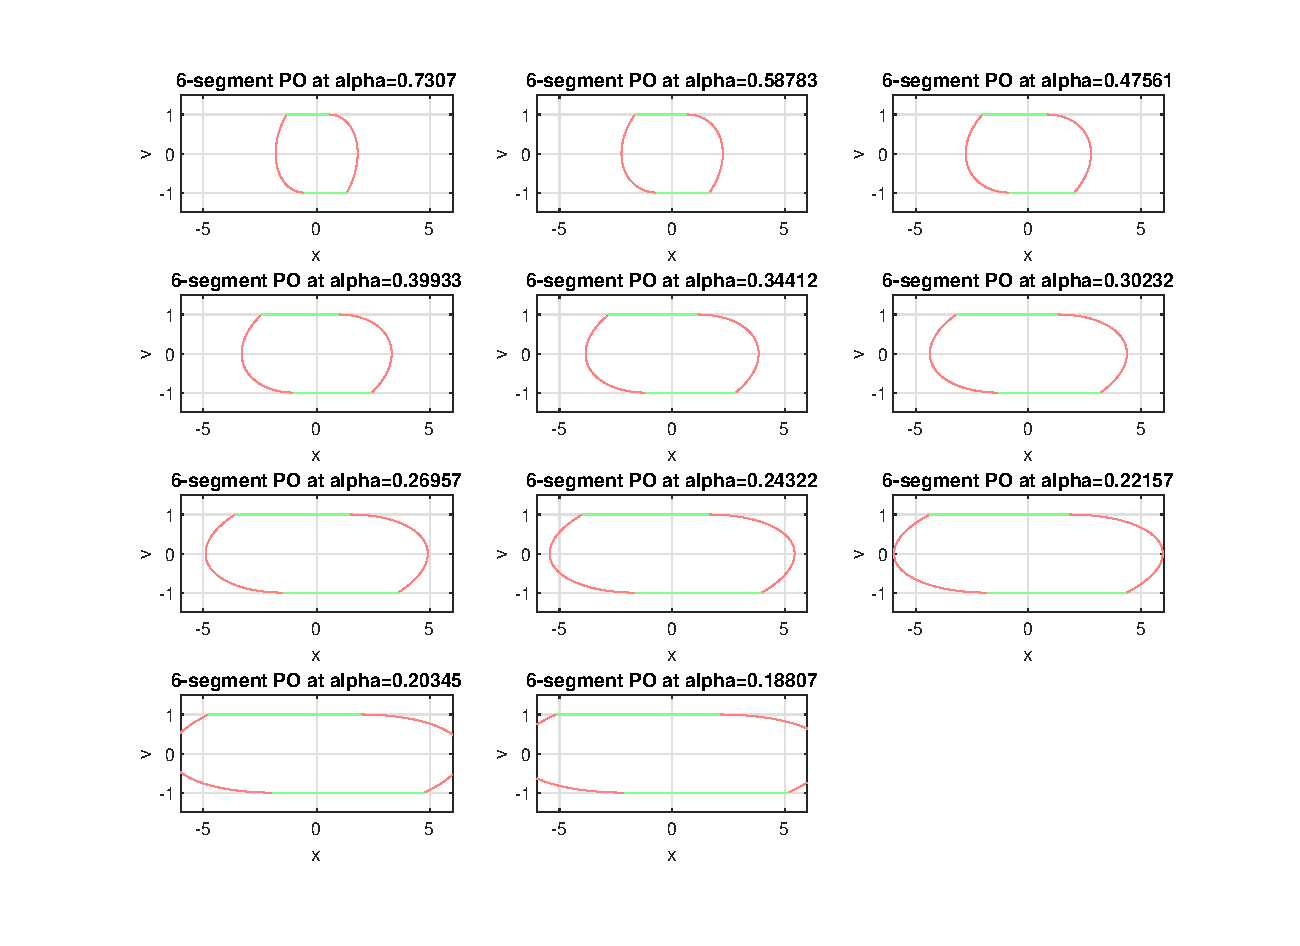
\includegraphics[height=10cm]{fig4}
	\caption{Family of 4-segment \emph{USUS} POs. \label{fig:4}}
\end{figure}

\newpage

\texttt{vector\_field\_.m} generates a figure which illustrates the vector field of the hybrid system, along with a 6-segment UCSUCS periodic orbit. It is clearly visible, that sliding mode starts, when the vector field of both (U) and (C) lead towards the switching line and ends when the dynamics of (U) becomes parallel to the switching line.

\begin{figure}[h!]
	\centering 
	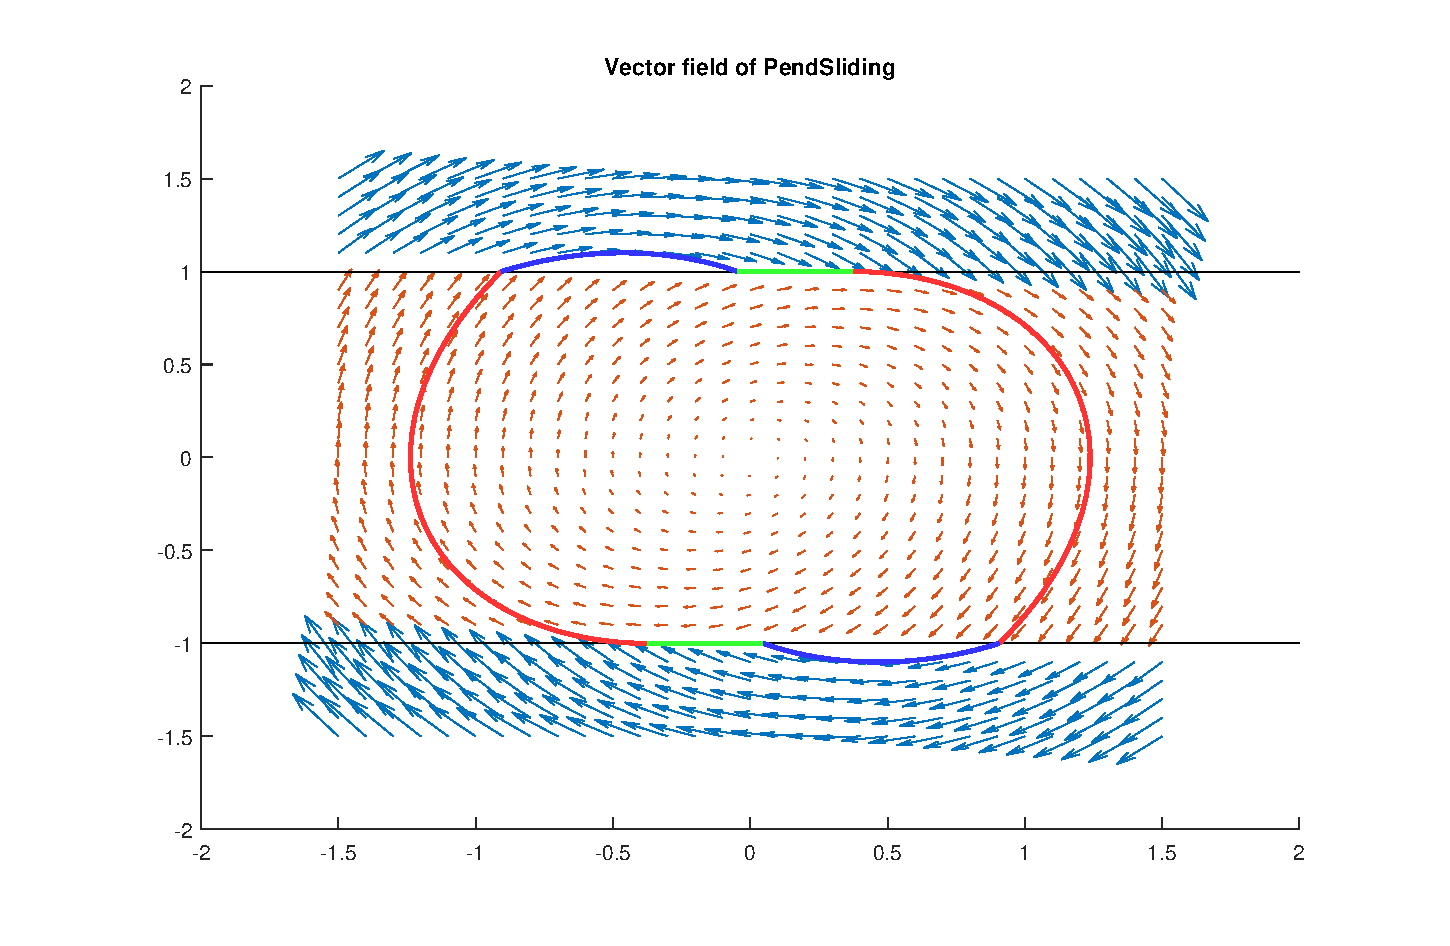
\includegraphics[height=8cm]{fig5}
	\caption{The vector field of the hybrid system and a 6-segment PO.\label{fig:5}}
\end{figure}

\end{document}